\documentclass[11pt, a4paper]{report}

% Encoding & lingua
\usepackage[utf8]{inputenc}
\usepackage[T1]{fontenc}
\usepackage[italian]{babel}
\usepackage{underscore}
\usepackage{lmodern}

% Impaginazione e tipografia
\usepackage[
  top=2.5cm, bottom=2.5cm,
  left=2.6cm,  right=2.6cm
]{geometry}
\usepackage[expansion=false]{microtype}
\usepackage{setspace}
\onehalfspacing
\raggedbottom

% Matematica
\usepackage{amsmath, amssymb, amsthm}
\usepackage{mathtools}
\usepackage[shortlabels]{enumitem}
\usepackage{bm}
\usepackage{booktabs}
\usepackage{graphicx}
\usepackage{needspace}

% Grafica TikZ per diagrammi vettoriali perfetti
\usepackage{tikz}
\usetikzlibrary{arrows.meta, positioning, shapes.geometric, automata, backgrounds, fit}

% tcolorbox per box pedagogici
\usepackage{tcolorbox}
\tcbuselibrary{skins, breakable}

% Hyperref
\usepackage[colorlinks=true, linkcolor=blue!70!black, citecolor=blue!70!black, urlcolor=blue!70!black]{hyperref}

% Ambienti Teorema Standard
\theoremstyle{plain}
\newtheorem{theorem}{Teorema}[chapter]
\newtheorem{proposition}[theorem]{Proposizione}
\newtheorem{lemma}[theorem]{Lemma}
\newtheorem{corollary}[theorem]{Corollario}
\theoremstyle{definition}
\newtheorem{definition}[theorem]{Definizione}
\newtheorem{esempio}[theorem]{Esempio}
\theoremstyle{remark}
\newtheorem{remark}[theorem]{Osservazione}

% Box Pedagogici con tcolorbox per Studio Orale (con break pulito)
\newtcolorbox{spiegazione}[1][In parole semplici (L'Intuizione)]{
  enhanced,
  breakable,
  pad at break=2mm,
  bottomrule at break=0mm,
  toprule at break=0mm,
  colback=green!5!white,
  colframe=green!60!black,
  fonttitle=\bfseries\sffamily,
  title={$\blacktriangleright$ Intuizione: #1},
  arc=2.5mm,
  boxrule=1pt,
  left=3.5mm, right=3.5mm, top=2.5mm, bottom=2.5mm,
  before skip=10pt, after skip=10pt
}

\newtcolorbox{hint}[1][Suggerimento Pratico]{
  enhanced,
  breakable,
  pad at break=2mm,
  bottomrule at break=0mm,
  toprule at break=0mm,
  colback=blue!5!white,
  colframe=blue!50!black,
  fonttitle=\bfseries\sffamily,
  title={$\blacktriangleright$ Suggerimento: #1},
  arc=2.5mm,
  boxrule=1pt,
  left=3.5mm, right=3.5mm, top=2.5mm, bottom=2.5mm,
  before skip=10pt, after skip=10pt
}

\newtcolorbox{domandaprof}[1][Cosa Chiede il Prof all'Orale]{
  enhanced,
  breakable,
  pad at break=2mm,
  bottomrule at break=0mm,
  toprule at break=0mm,
  colback=yellow!6!white,
  colframe=orange!85!black,
  fonttitle=\bfseries\sffamily,
  title={$\blacktriangleright$ Domanda del Prof: #1},
  arc=2.5mm,
  boxrule=1pt,
  left=3.5mm, right=3.5mm, top=2.5mm, bottom=2.5mm,
  before skip=10pt, after skip=10pt
}

\newtcolorbox{lavagna}[1][Traccia Passo-Passo per la Lavagna]{
  enhanced,
  breakable,
  pad at break=2mm,
  bottomrule at break=0mm,
  toprule at break=0mm,
  colback=purple!5!white,
  colframe=purple!70!black,
  fonttitle=\bfseries\sffamily,
  title={$\blacktriangleright$ Dimostrazione alla Lavagna: #1},
  arc=2.5mm,
  boxrule=1pt,
  left=3.5mm, right=3.5mm, top=2.5mm, bottom=2.5mm,
  before skip=10pt, after skip=10pt
}

\newtcolorbox{trappola}[1][Attenzione: Trabocchetto Tipico]{
  enhanced,
  breakable,
  pad at break=2mm,
  bottomrule at break=0mm,
  toprule at break=0mm,
  colback=red!5!white,
  colframe=red!70!black,
  fonttitle=\bfseries\sffamily,
  title={$\blacktriangleright$ Attenzione / Trabocchetto: #1},
  arc=2.5mm,
  boxrule=1pt,
  left=3.5mm, right=3.5mm, top=2.5mm, bottom=2.5mm,
  before skip=10pt, after skip=10pt
}

\newtcolorbox{sirlink}[1][Collegamento al Progetto SIR]{
  enhanced,
  breakable,
  pad at break=2mm,
  bottomrule at break=0mm,
  toprule at break=0mm,
  colback=blue!5!white,
  colframe=blue!70!black,
  fonttitle=\bfseries\sffamily,
  title={$\blacktriangleright$ Collegamento al Progetto SIR: #1},
  arc=2.5mm,
  boxrule=1pt,
  left=3.5mm, right=3.5mm, top=2.5mm, bottom=2.5mm,
  before skip=10pt, after skip=10pt
}

% Macro Matematiche
\newcommand{\PP}{\mathbb{P}}
\newcommand{\E}{\mathbb{E}}
\newcommand{\F}{\mathcal{F}}
\newcommand{\G}{\mathcal{G}}
\newcommand{\R}{\mathbb{R}}
\newcommand{\N}{\mathbb{N}}
\newcommand{\QQ}{\mathbb{Q}}
\newcommand{\1}{\mathbf{1}}
\newcommand{\Var}{\operatorname{Var}}
\newcommand{\Cov}{\operatorname{Cov}}

\begin{document}

\title{
  \Huge\textbf{Modelli Probabilistici per le Applicazioni}\\
  \vspace{0.4cm}
  \LARGE\textbf{Dispense Complete di Studio \& Orale con Figure}\\
  \vspace{0.2cm}
  \large\textit{Versione Definitiva Illustrata per Informatica: Teoria Integrale, Esercizi, Schemi Grafici TikZ, Spiegazioni Intuitive, Domande del Docente e Prove alla Lavagna}
}
\author{\textbf{Francesco Castaldi} (\texttt{francesco.castaldi4@studio.unibo.it})\\Corso di Laurea in Informatica — Università di Bologna\\Docente: Prof. Salvatore Federico}
\date{Anno Accademico 2025/2026}

\maketitle

\begin{abstract}
Questo testo raccoglie la trattazione teorica integrale e dettagliata per la preparazione della prova orale dell'insegnamento di \emph{Modelli Probabilistici} (518512). Il contenuto rispetta rigorosamente il programma ufficiale per il Corso di Laurea in Informatica stabilito dal Prof. Salvatore Federico, escludendo i due capitoli non previsti (\emph{Finanza Matematica} e \emph{Controllo Stocastico}) e mantenendo intatta tutta la profondità formale delle dispense d'origine (definizioni, teoremi, dimostrazioni ed esercizi d'esame). Il testo è arricchito con spiegazioni a parole semplici, schemi grafici vettoriali TikZ, figure ad alta risoluzione del simulatore, box di intuizione fisica, schede di risposta alle domande tipiche del docente, tracce per la lavagna e collegamenti al progetto pratico della Catena di Markov del modello epidemiologico SIR.
\end{abstract}

\tableofcontents
\newpage

% =========================================================================
% INTRODUZIONE & STRATEGIA D'ESAME
% =========================================================================
\chapter*{Guida alla Prova Orale \& Strategia d'Esame}
\addcontentsline{toc}{chapter}{Guida alla Prova Orale \& Strategia d'Esame}

La prova orale con il Prof. Salvatore Federico ha una durata indicativa di \textbf{25--30 minuti} ed è strutturata in due parti consecutive:

\begin{enumerate}
    \item \textbf{Parte 1 — Presentazione del Progetto SIR (10--15 minuti)}:
    \begin{itemize}
        \item Presentazione delle slide Beamer (o della versione stampabile A4 consegnata al docente).
        \item Esposizione della modellizzazione compartimentale stocastica discreta: spazio stati $\mathcal{S}$, estrazioni binomiali condizionate $C_t \sim \text{Bin}(S_t, \beta I_t/N)$ e $G_t \sim \text{Bin}(I_t, \gamma)$.
        \item Spiegazione delle proprietà della matrice di transizione $P$, degli stati assorbenti $I=0$, della monotonicità di $R_t$, del tempo medio di estinzione $\mathbb{E}[\tau]$ e del confronto con la ODE deterministica di Kermack--McKendrick.
    \end{itemize}
    
    \item \textbf{Parte 2 — Domande Teoriche sulle Dispense \& Lavagna (10--15 minuti)}:
    \begin{itemize}
        \item Domande di verifica concettuale su definizioni e teoremi delle dispense ufficiali.
        \item Richiesta di svolgere una \textbf{dimostrazione formale alla lavagna} o su foglio (es. equazioni di Chapman-Kolmogorov, proprietà della torre del valore atteso condizionale, conservazione della media per martingale, o calcolo del tempo medio di assorbimento).
    \end{itemize}
\end{enumerate}

\begin{spiegazione}[{La Struttura della Risposta Perfetta all'Orale}]
Quando il docente ti pone una domanda teorica, organizza sempre la risposta in 3 passaggi:
\begin{enumerate}
    \item \textbf{Sintesi intuitiva in una frase}: ``Intuitivamente questo concetto esprime che...''.
    \item \textbf{Definizione o Teorema Formale}: Enuncia la formula matematica rigorosa con tutte le ipotesi necessarie.
    \item \textbf{Esempio o Collegamento al Progetto}: ``Questo è esattamente ciò che abbiamo verificato sperimentalmente nel progetto quando...''.
\end{enumerate}
\end{spiegazione}

\newpage

% =========================================================================
% CAPITOLO 1: TEORIA DELLA PROBABILITA' IN SPAZI FINITI
% =========================================================================
\chapter{Teoria della probabilità in spazi finiti}

La teoria matematica della probabilità mira a costruire un formalismo teorico per descrivere i \emph{fenomeni aleatori} (casuali). Si basa sul concetto di \emph{esperimento aleatorio}, che può essere approssimativamente definito come ``un esperimento il cui risultato non può essere previsto in anticipo''. Un individuo può essere naturalmente portato ad associare un \emph{grado di fiducia} ai diversi possibili risultati di questo esperimento. Vediamo come modellizzare matematicamente questa idea, tenendo sempre presente che in ogni buona teoria vi sono tre fasi distinte:
\begin{enumerate}[(i)]
    \item Scelta del modello matematico;
    \item Elaborazione matematica all'interno del modello scelto;
    \item Interpretazione dei risultati ottenuti.
\end{enumerate}

\section{Spazi di probabilità}

La struttura degli spazi di probabilità si compone di tre ingredienti fondamentali:
\begin{enumerate}
    \item Lo spazio campionario (o spazio degli stati) $\Omega$;
    \item L'insieme degli eventi $\F$;
    \item La misura di probabilità $\PP$.
\end{enumerate}
Di conseguenza, uno spazio di probabilità è una terna: $(\Omega, \F, \PP)$. Descriviamo nel dettaglio gli oggetti di questa terna.

\begin{hint}[{La Terna Fondamentale}]
    Per ricordare la terna $(\Omega, \F, \PP)$:
    \begin{itemize}
        \item $\Omega$ (Omega) è \textbf{TUTTO} quello che può succedere (lo Spazio).
        \item $\F$ (F corsiva) sono le \textbf{DOMANDE} che puoi fare (gli Eventi a cui puoi assegnare una probabilità).
        \item $\PP$ (P) è la \textbf{RISPOSTA} (la Misura, il numero da 0 a 1).
    \end{itemize}
\end{hint}

\subsection{Spazio campionario \texorpdfstring{($\Omega$)}{(Omega)}}

Lo \emph{spazio campionario} è l'insieme i cui elementi rappresentano tutti i possibili ``stati futuri/sconosciuti del mondo'' \emph{mutuamente esclusivi}. È tradizionalmente indicato con $\Omega$ e il suo elemento generico è indicato con $\omega$. In questo capitolo assumiamo che lo spazio campionario $\Omega$ sia finito, ovvero $|\Omega| < \infty$. Naturalmente questa è un'assunzione restrittiva, ma ci permette comunque di modellare molti fenomeni.

\begin{esempio}[Monete e Dadi]
    \begin{itemize}
        \item \textbf{Lancio di una moneta:} Una scelta ragionevole per lo spazio campionario è $\Omega = \{T, C\}$ (Testa, Croce) oppure $\Omega = \{0, 1\}$. Le etichette non sono importanti.
        \item \textbf{Due lanci di una moneta (o lancio di due monete):} Una scelta logica è elencare le coppie: $\Omega := \{(T, T), (T, C), (C, T), (C, C)\}$.
        \item \textbf{Lancio di due dadi a sei facce:} $\Omega := \{(i, j) : i, j \in \{1, 2, 3, 4, 5, 6\}\}$. Si noti che $|\Omega| = 36$.
    \end{itemize}
\end{esempio}

\subsection{Spazio degli eventi \texorpdfstring{($\F$)}{(F)}}

Matematicamente, un \emph{evento} è un sottoinsieme $A \subseteq \Omega$ di risultati $\omega$. Interpretiamo $A$ come un evento che \emph{si è verificato} se il risultato effettivo $\omega \in A$, e che \emph{non si è verificato} se $\omega \notin A$. Questa rappresentazione matematica ci permette di tradurre domande intuitive in operazioni insiemistiche precise:
\begin{itemize}
    \item L'evento $\Omega$ è l'evento \emph{certo}.
    \item L'evento $\emptyset$ è l'evento \emph{impossibile}.
    \item Il singoletto $\{\omega\}$ è un evento \emph{elementare}.
    \item Dato $A \subseteq \Omega$, $A^c$ è l'``evento complementare (o contrario) di $A$''.
    \item L'unione $A \cup B$ è l'evento ``$A$ e/o $B$ si verificano''.
    \item L'intersezione $A \cap B$ è l'evento ``Sia $A$ che $B$ si verificano contemporaneamente''.
\end{itemize}

L'insieme di tutti gli eventi di interesse è solitamente denotato con $\F$. Questo insieme deve avere delle ``proprietà di stabilità'', ovvero deve essere un'\emph{algebra}.

\begin{definition}[Algebra di insiemi e atomi]
Un insieme di sottoinsiemi $\F \subseteq 2^\Omega$ è chiamato \emph{algebra (di insiemi)} se valgono le seguenti proprietà:
\begin{enumerate}[(F1)]
    \item $\Omega \in \F$;
    \item $A \in \F \implies A^c \in \F$;
    \item $A, B \in \F \implies A \cup B \in \F$.
\end{enumerate}
Se $\F$ è un'algebra, un insieme $A \in \F$ è chiamato \emph{atomo} di $\F$ se non può essere decomposto come unione di due insiemi non vuoti e disgiunti di $\F$.
\end{definition}

\begin{spiegazione}[{Perché ci serve un'algebra?}]
    Perché se possiamo chiederci qual è la probabilità che piova (evento $A$), dobbiamo poterci chiedere anche qual è la probabilità che NON piova (evento $A^c$), oppure che piova o nevichi ($A \cup B$). L'algebra garantisce che il nostro ``vocabolario'' di eventi sia logicamente completo.
\end{spiegazione}

\subsection{Misura di probabilità \texorpdfstring{($\PP$)}{(P)}}

Una volta fissato lo spazio degli eventi $\F$, ad ogni evento $A \in \F$ si può associare un ``grado di fiducia'' chiamato \emph{probabilità dell'evento A}. Questo è formalizzato da una funzione:
\[ \PP : \F \to [0, 1] \]
La scelta di questa misura è soggettiva, ma deve rispettare i ``tre assiomi della probabilità'' per escludere scelte illogiche.

\begin{definition}[Misura di probabilità]
Sia $\Omega$ un insieme finito e sia $\F \subseteq 2^\Omega$ un'algebra. Una \emph{misura di probabilità} su $\F$ è una mappa $\PP : \F \to \R$ tale che:
\begin{enumerate}[(A1)]
    \item $0 \le \PP(A) \le 1$ per ogni $A \in \F$;
    \item $\PP(\Omega) = 1$;
    \item $A, B \in \F$ con $A \cap B = \emptyset \implies \PP(A \cup B) = \PP(A) + \PP(B)$.
\end{enumerate}
\end{definition}

\begin{hint}[{Additività}]
    L'assioma (A3) è la \textbf{Regola della Somma}: se due eventi non possono verificarsi insieme (sono disgiunti), la probabilità che se ne verifichi almeno uno è la somma delle loro probabilità singole. (Es. Probabilità di tirare 1 o 2 con un dado = $\PP(1) + \PP(2)$).
\end{hint}

Dagli assiomi derivano proprietà utilissime:
\begin{itemize}
    \item $\PP(A^c) = 1 - \PP(A)$
    \item Se $A \subseteq B$, allora $\PP(B \setminus A) = \PP(B) - \PP(A)$ e quindi $\PP(A) \le \PP(B)$.
    \item $\PP(A \cup B) = \PP(A) + \PP(B) - \PP(A \cap B)$
\end{itemize}

\section{Variabili aleatorie}

Nelle applicazioni pratiche, spesso non ci interessa l'esito esatto $\omega$, ma un numero o una quantità derivata da esso (es. la somma di due dadi, il guadagno in un gioco). Questo ci porta alle variabili aleatorie.

\begin{definition}[Variabile aleatoria]
Sia dato uno spazio $(\Omega, \F)$. Una mappa $X : \Omega \to E$ è una \emph{variabile aleatoria} se è $\F$-misurabile, ovvero se:
\[ X^{-1}(B) := \{X \in B\} \in \F \quad \forall B \subseteq E \]
\end{definition}

In spazi campionari finiti in cui $\F = 2^\Omega$, \textbf{ogni funzione $X$ è una variabile aleatoria}.

\begin{spiegazione}[{Cos'è una variabile aleatoria in parole povere}]
    Una variabile aleatoria non è né una ``variabile'' in senso stretto, né tantomeno ``aleatoria'' (casuale). È semplicemente una \textbf{funzione deterministica} che prende in input lo stato del mondo $\omega$ (quello sì che è casuale) e restituisce un valore, di solito un numero. \\
    Esempio: se $\omega = (\text{Testa}, \text{Testa})$, la variabile aleatoria $X = \text{``numero di teste''}$ restituirà banalmente $X(\omega) = 2$.
\end{spiegazione}

\subsection{Misurabilità di una mappa e algebra generata}

\begin{definition}[Algebra generata $\sigma(X)$]
Sia $X : \Omega \to E$ una variabile aleatoria. L'\emph{algebra generata} da $X$, denotata con $\sigma(X)$, è la più piccola algebra su $\Omega$ che rende $X$ misurabile:
\[ \sigma(X) := \{ X^{-1}(B) : B \subseteq E \} \]
\end{definition}

Gli atomi di $\sigma(X)$ sono esattamente gli insiemi di livello $\{X = x\}$ per ogni $x \in E$. 
\textbf{Intuizione:} L'algebra $\sigma(X)$ rappresenta tutta l'informazione che deduco osservando $X$.

\begin{theorem}[Criterio di misurabilità di Doob]
Siano $X : \Omega \to E$ e $Y : \Omega \to E'$ variabili aleatorie. 
$X$ è $\sigma(Y)$-misurabile se e solo se esiste una funzione $f : E' \to E$ tale che $X = f \circ Y$.
\end{theorem}

\begin{hint}[{Interpretare Doob}]
    Cosa significa che $X$ è $\sigma(Y)$-misurabile? 
    Significa che \textbf{l'informazione fornita da $Y$ è sufficiente a determinare $X$}. Se conosco $Y$, conosco automaticamente anche $X$. 
    Perché? Perché se $X = f(Y)$, basta applicare la funzione deterministica $f$ al valore di $Y$ per trovare $X$. Se invece serve lanciare una moneta aggiuntiva, allora $X$ \textbf{non} è $\sigma(Y)$-misurabile.
\end{hint}

\subsection{Legge (o distribuzione) di una variabile aleatoria}

\begin{definition}[Legge o distribuzione]
Data una variabile aleatoria $X : \Omega \to E$, possiamo trasferire la misura di probabilità da $(\Omega, \F, \PP)$ allo spazio dei valori $(E, 2^E)$ definendo:
\[ \mu_X(B) := \PP(X \in B) \quad \forall B \subseteq E \]
Questa nuova misura di probabilità si chiama \emph{legge} o \emph{distribuzione} di $X$.
La funzione $f_X(x) := \PP(X = x)$ è la sua \emph{funzione di densità discreta}.
\end{definition}

\subsection{Distribuzione congiunta e distribuzioni marginali}

\begin{definition}[Leggi congiunte e marginali]
Date $n$ variabili aleatorie $X_j : \Omega \to E_j$, con $j=1,\dots,n$, il vettore $X = (X_1, \dots, X_n)$ è una variabile aleatoria a valori in $E = E_1 \times \dots \times E_n$.
La \emph{legge congiunta} $\mu_X = L(X_1, \dots, X_n)$ è la misura di probabilità definita da:
\[ \mu_X(A_1 \times \dots \times A_n) := \PP(X_1 \in A_1, \dots, X_n \in A_n) \]
Le \emph{densità discrete marginali} si ottengono sommando rispetto a tutte le altre variabili:
\[ f_{X_i}(x_i) = \sum_{x_1, \dots, x_{i-1}, x_{i+1}, \dots, x_n} f_X(x_1, \dots, x_n) \]
\end{definition}

\begin{spiegazione}[{Congiunta e Marginale}]
    Immagina la legge congiunta come una grande tabella a doppia entrata. Le celle interne contengono la probabilità che $X=x$ e $Y=y$ contemporaneamente. 
    Se sommiamo tutti i valori di una riga, troviamo la probabilità totale di $X=x$ (a prescindere da $Y$). Questa somma ``ai margini'' della tabella è la \emph{distribuzione marginale}.
\end{spiegazione}

\section{Probabilità Condizionata e Bayes}

\begin{definition}[Probabilità Condizionata]
Dato uno spazio di probabilità $(\Omega, \F, \PP)$ e un evento $H \in \F$ con $\PP(H) > 0$:
\[ \PP(A|H) := \frac{\PP(A \cap H)}{\PP(H)} \]
\end{definition}

\subsection{Legge della probabilità totale e Teorema di Bayes}

\begin{figure}[htbp]
\centering
\begin{tikzpicture}[scale=0.88]
  % Omega box
  \draw[thick, rounded corners=3mm, fill=blue!3, draw=blue!50!black] (-4.5,-2.2) rectangle (4.5,2.2);
  \node[font=\bfseries, text=blue!70!black] at (4.0, 1.8) {$\Omega$};
  % Partitions
  \draw[dashed, blue!60!black, thick] (-1.5,-2.2) -- (-1.5,2.2);
  \draw[dashed, blue!60!black, thick] (1.5,-2.2) -- (1.5,2.2);
  \node[blue!80!black, font=\bfseries] at (-3.0, 1.7) {Partizione $A_1$};
  \node[blue!80!black, font=\bfseries] at (0, 1.7) {Partizione $A_2$};
  \node[blue!80!black, font=\bfseries] at (3.0, 1.7) {Partizione $A_3$};
  % Event B
  \draw[thick, fill=red!20, fill opacity=0.7, draw=red!70!black] (0, -0.4) ellipse (2.8cm and 1.3cm);
  \node[red!90!black, font=\bfseries\large] at (0, 0.4) {Evento $B$};
  \node[font=\footnotesize\bfseries, text=red!80!black] at (-2.2, -0.4) {$B \cap A_1$};
  \node[font=\footnotesize\bfseries, text=red!80!black] at (0, -0.8) {$B \cap A_2$};
  \node[font=\footnotesize\bfseries, text=red!80!black] at (2.2, -0.4) {$B \cap A_3$};
\end{tikzpicture}
\caption{Rappresentazione geometrica della Legge della Probabilità Totale: l'evento $B$ viene ``disintegrato'' nelle sue intersezioni disgiunte con i blocchi della partizione $\{A_1, A_2, A_3\}$.}
\label{fig:prob_totale}
\end{figure}

\begin{theorem}[{Probabilità totale e Bayes}]
\begin{enumerate}
    \item \textbf{Legge della probabilità totale}: Se $A_1, \dots, A_n$ formano una partizione di $\Omega$:
    \[ \PP(B) = \sum_{i=1}^n \PP(A_i) \PP(B|A_i) \]
    \item \textbf{Teorema di Bayes}: Per due eventi $A$ e $B$ con $\PP(A)>0$ e $\PP(B)>0$:
    \[ \PP(A|B) = \frac{\PP(B|A)\PP(A)}{\PP(B)} = \frac{\PP(B|A)\PP(A)}{\sum_{j=1}^n \PP(B|A_j)\PP(A_j)} \]
\end{enumerate}
\end{theorem}

\begin{spiegazione}[{Bayes e Probabilità Totale}]
    \textbf{Probabilità Totale}: Se voglio calcolare la probabilità che piova (evento B), posso dividere il mondo in scenari (partizione): $A_1$=è nuvoloso, $A_2$=è sereno. La probabilità che piova sarà la probabilità che piova QUANDO è nuvoloso per la probabilità che sia nuvoloso, PIÙ la probabilità che piova QUANDO è sereno per la probabilità che sia sereno. \\
    \textbf{Bayes}: Serve a ``ribaltare'' la domanda. Conosciamo la probabilità di avere un test positivo sapendo di essere malati $\PP(+|\text{Malato})$, ma a noi interessa la probabilità di essere malati avendo il test positivo $\PP(\text{Malato}|+)$! Bayes fa esattamente questo.
\end{spiegazione}

\section{Indipendenza}

\begin{definition}[Indipendenza tra variabili aleatorie ed eventi]
Due variabili aleatorie $X$ e $Y$ sono \emph{indipendenti} se per ogni evento $\{Y \in B\}$ con $\PP(Y \in B)>0$:
\[ \PP(X \in A \mid Y \in B) = \PP(X \in A) \iff \PP(X \in A, Y \in B) = \PP(X \in A)\PP(Y \in B) \]
Due eventi $A, B \in \F$ sono indipendenti se e solo se $\PP(A \cap B) = \PP(A)\PP(B)$.
\end{definition}

\begin{domandaprof}[{Indipendenza vs Incorrelazione}]
\textbf{Il Prof chiede}: ``Se due variabili hanno covarianza nulla $\Cov(X,Y)=0$, sono indipendenti?''.\\
\textbf{Risposta esatta}: \textbf{NO!} L'indipendenza implica sempre covarianza nulla, ma l'inverso è falso in generale.\\
\textbf{Controesempio immediato}: Sia $X$ uniforme su $\{-1, 0, 1\}$ e sia $Y = X^2$.
\begin{itemize}
    \item $X$ e $Y$ sono palesemente \textbf{dipendenti} ($Y$ è deterministica in $X$).
    \item Calcolando la covarianza: $\E[X] = 0$, $\E[X Y] = \E[X^3] = 0$. Dunque $\Cov(X,Y) = \E[XY] - \E[X]\E[Y] = 0 - 0 = 0$.
\end{itemize}
\end{domandaprof}

\section{Valore Atteso e Valore Atteso Condizionato}

\begin{definition}[Valore atteso]
Sia $X : \Omega \to \R$ una variabile aleatoria. Il suo valore atteso è:
\[ \E[X] := \sum_{x \in E} x \PP(X = x) \]
\end{definition}

\begin{definition}[Valore atteso condizionato rispetto a una variabile $Y$]
$\E[X|Y]$ è la variabile aleatoria definita da $\E[X|Y](\omega) = \E[X \mid Y = Y(\omega)]$.
\end{definition}

Proprietà fondamentali di $\E[X|Y]$:
\begin{itemize}
    \item Se $X$ e $Y$ sono indipendenti: $\E[X|Y] = \E[X]$.
    \item Se $X$ è determinata da $Y$ ($X = f(Y)$): $\E[X|Y] = X$.
    \item \textbf{Legge delle aspettative iterate (Tower property)}: $\E[\E[X|Y]] = \E[X]$.
    \item \textbf{Freezing Lemma}: $\E[\phi(X,Y)|Y](\omega) = \E[\phi(X, y)]\big|_{y=Y(\omega)}$.
\end{itemize}

\newpage

% =========================================================================
% CAPITOLO 2: IL CASO DISCRETO GENERALE
% =========================================================================
\chapter{Il caso discreto: da finito a numerabile}

Fino ad ora abbiamo considerato solo spazi di probabilità finiti. Questo è un limite significativo per descrivere molti fenomeni naturali (es. tempi d'attesa non limitati a priori o processi su orizzonte temporale infinito).
Dobbiamo estendere il nostro quadro teorico agli spazi numerabili.

\section{Spazi di probabilità generali}

\begin{definition}[$\sigma$-algebra]
Una collezione $\F \subseteq 2^\Omega$ è chiamata \emph{$\sigma$-algebra} su $\Omega$ se:
\begin{enumerate}
    \item $\Omega \in \F$,
    \item $A \in \F \implies A^c \in \F$,
    \item Per ogni collezione numerabile $\{A_n\}_{n \in \N} \subseteq \F$, l'unione $\bigcup_{n \in \N} A_n \in \F$.
\end{enumerate}
\end{definition}

\begin{definition}[Misura di probabilità ($\sigma$-additiva)]
Sia $\F$ una $\sigma$-algebra. Una funzione $\PP : \F \to [0, 1]$ è una \emph{misura di probabilità} su $(\Omega, \F)$ se:
\begin{enumerate}
    \item $0 \le \PP(A) \le 1$ per ogni $A \in \F$,
    \item $\PP(\Omega) = 1$,
    \item \textbf{$\sigma$-additività}: per ogni collezione numerabile di eventi disgiunti $\{A_n\}_{n \in \N}$:
    \[ \PP\left(\bigcup_{n=1}^\infty A_n\right) = \sum_{n=1}^\infty \PP(A_n) \]
\end{enumerate}
\end{definition}

\section{Distribuzioni Notevoli Discrete}

\subsection{Distribuzione di Poisson}
$X \sim \mathcal{P}(\lambda)$ con $\lambda > 0$: $\PP(X = k) = e^{-\lambda} \frac{\lambda^k}{k!}$ per $k \in \N_0$. Vale $\E[X] = \lambda$ e $\Var(X) = \lambda$.

\subsection{Distribuzione Geometrica e Assenza di Memoria}
$T \sim \text{Geom}(p)$ modella il tempo di primo successo: $\PP(T = n) = (1-p)^{n-1} p$ per $n \ge 1$.
\begin{theorem}[Proprietà di Assenza di Memoria]
\[ \PP(T = n + k \mid T > n) = \PP(T = k) \quad \forall n, k \ge 1 \]
\end{theorem}

\section{Disuguaglianze Notevoli e Valore Atteso}

\begin{theorem}[Disuguaglianze di Markov e Chebyshev]
\textbf{Markov:} Per ogni $X \ge 0$ e $a > 0$: $\PP(X \ge a) \le \frac{\E[X]}{a}$.\\
\textbf{Chebyshev:} Per ogni $X$ con media $m$ e varianza finita $\sigma^2$: $\PP(|X - m| \ge \epsilon) \le \frac{\sigma^2}{\epsilon^2}$.
\end{theorem}

\section{Convergenze di Variabili Aleatorie}

\begin{definition}[Tipi di Convergenza]
\begin{enumerate}
    \item \textbf{Quasi Certamente (a.s.)}: $\PP(\lim_{n\to\infty} X_n = X) = 1$.
    \item \textbf{In Probabilità}: $\forall \epsilon > 0$, $\lim_{n\to\infty} \PP(|X_n - X| \ge \epsilon) = 0$.
    \item \textbf{In Legge}: Per ogni $\phi$ limitata e continua, $\E[\phi(X_n)] \to \E[\phi(X)]$.
\end{enumerate}
\end{definition}

\begin{spiegazione}[{Gerarchia delle Convergenze}]
    \[ \text{Quasi Certamente} \implies \text{In Probabilità} \implies \text{In Legge} \]
    Le implicazioni inverse non valgono in generale!
\end{spiegazione}

\subsection{Teoremi di Passaggio al Limite sotto Segno di Media}
\begin{itemize}
    \item \textbf{Beppo-Levi (Monotona)}: Se $0 \le X_n \uparrow X$ q.c., allora $\lim \E[X_n] = \E[X]$.
    \item \textbf{Lemma di Fatou}: Se $X_n \ge 0$, allora $\E[\liminf X_n] \le \liminf \E[X_n]$.
    \item \textbf{Lebesgue (Convergenza Dominata)}: Se $X_n \to X$ q.c. e $|X_n| \le G \in L^1$, allora $\lim \E[X_n] = \E[X]$.
\end{itemize}

\section{Legge dei Grandi Numeri}

\begin{theorem}[Legge debole e forte dei grandi numeri]
Sia $(X_n)$ i.i.d. con media $m$ e varianza $\sigma^2 < \infty$. Posto $\bar{S}_n = \frac{1}{n}\sum_{i=1}^n X_i$:
\begin{itemize}
    \item \textbf{Legge Debole}: $\bar{S}_n \stackrel{P}{\to} m$ in probabilità (dimostrata via Chebyshev).
    \item \textbf{Legge Forte}: $\bar{S}_n \to m$ quasi certamente.
\end{itemize}
\end{theorem}

\section{Esercizi Selezionati (Capitolo 2)}
\begin{itemize}
    \item \textbf{Esercizio 1 (Tempi d'attesa dispari)}: Per $T \sim \text{Geom}(1/2)$, $\PP(T \in \text{dispari}) = \sum_{k=0}^\infty (1/2)^{2k+1} = \frac{2}{3}$.
    \item \textbf{Esercizio 2 (Stop al disaccordo)}: Per estrazioni binarie da urne, la durata $N \sim \text{Geom}(2p(1-p))$ è \textbf{indipendente} dall'esito della vincita $V \sim \mathcal{B}(1/2)$.
    \item \textbf{Esercizio 3 (Successi intermedi)}: Dato $T_2=N$, il tempo del primo successo $T_1$ è uniforme su $\{1, \dots, N-1\}$.
    \item \textbf{Esercizio 5 (Poisson split)}: Se $N \sim \mathcal{P}(\lambda)$ e $X_i \sim \mathcal{B}(p)$, allora $S_N \sim \mathcal{P}(\lambda p)$ e $N - S_N \sim \mathcal{P}(\lambda(1-p))$ sono \textbf{indipendenti}.
\end{itemize}

\newpage

% =========================================================================
% CAPITOLO 3: PROCESSI STOCASTICI A TEMPO DISCRETO
% =========================================================================
\chapter{Processi stocastici a tempo discreto}

\section{Nozione di Processo Stocastico e Filtrazioni}

Un processo stocastico è una famiglia $X = (X_n)_{n \in \N_0}$ di variabili aleatorie a valori in uno spazio discreto $E$.

\begin{figure}[htbp]
\centering
\begin{tikzpicture}[
  level 1/.style={sibling distance=5cm, level distance=1.6cm},
  level 2/.style={sibling distance=2.5cm, level distance=1.6cm},
  every node/.style={circle, draw=blue!70!black, fill=blue!10, inner sep=2.5pt, font=\footnotesize\bfseries},
  edge from parent/.style={draw=blue!60!black, -Latex, thick}
]
  \node {$\mathcal{F}_0$}
    child { node {$T$}
      child { node {$TT$} edge from parent node[left, draw=none, fill=none, font=\scriptsize] {$T$} }
      child { node {$TC$} edge from parent node[right, draw=none, fill=none, font=\scriptsize] {$C$} }
      edge from parent node[above left, draw=none, fill=none, font=\scriptsize] {$T$}
    }
    child { node {$C$}
      child { node {$CT$} edge from parent node[left, draw=none, fill=none, font=\scriptsize] {$T$} }
      child { node {$CC$} edge from parent node[right, draw=none, fill=none, font=\scriptsize] {$C$} }
      edge from parent node[above right, draw=none, fill=none, font=\scriptsize] {$C$}
    };
  \node[draw=none, fill=none, font=\small\bfseries, text=gray!80!black, right=3.8cm of {0,0}] {$t=0: \mathcal{F}_0 = \{\emptyset, \Omega\}$ (Informazione iniziale)};
  \node[draw=none, fill=none, font=\small\bfseries, text=gray!80!black, right=3.8cm of {0,-1.6}] {$t=1: \mathcal{F}_1 = \sigma(X_1)$ (2 rami)};
  \node[draw=none, fill=none, font=\small\bfseries, text=gray!80!black, right=3.8cm of {0,-3.2}] {$t=2: \mathcal{F}_2 = \sigma(X_1, X_2)$ (4 atomi)};
\end{tikzpicture}
\caption{Struttura ad albero di una filtrazione naturale $(\mathcal{F}_n)_{n \ge 0}$: ad ogni istante temporale l'algebra si arricchisce di nuovi atomi, rappresentando l'accumulo di informazione storica.}
\label{fig:filtrazione}
\end{figure}

\begin{definition}[Filtrazione Naturale e Processo Adattato]
La \emph{filtrazione naturale} è la famiglia crescente $\F_n^\xi = \sigma(\xi_0, \dots, \xi_n)$. Un processo $X$ è \emph{adattato} se ogni $X_n$ è $\F_n$-misurabile (non usa informazioni future).
\end{definition}

\section{Tempi di Arresto (Stopping Times)}

\begin{definition}[Tempo di arresto]
$\tau : \Omega \to \N_0 \cup \{\infty\}$ è un \emph{tempo di arresto} se $\{\tau \le n\} \in \F_n$ (ovvero $\{\tau = n\} \in \F_n$).
\end{definition}

\begin{spiegazione}[{Il tempo di arresto in parole semplici}]
    Un tempo di arresto è una regola per fermare un esperimento basandosi \textbf{solo su ciò che è accaduto fino ad oggi}, senza poteri divinatori sul futuro.
    \begin{itemize}
        \item ``Fermati non appena perdi 10 euro'' $\to$ \textbf{È uno stopping time} (puoi controllarlo giorno per giorno).
        \item ``Fermati il giorno prima del massimo rialzo della borsa'' $\to$ \textbf{NON è uno stopping time} (richiede di conoscere il futuro!).
    \end{itemize}
\end{spiegazione}

\newpage

% =========================================================================
% CAPITOLO 4: MARTINGALE
% =========================================================================
\chapter{Martingale}

\section{Nozione di Martingala}

\begin{definition}[Martingala, Submartingala, Supermartingala]
Sia $X = (X_n)_{n \in \N_0}$ un processo reale adattato a $(\F_n)$ con $X_n \in L^1$.
\begin{itemize}
    \item \textbf{Submartingala}: $\E[X_{n+1} \mid \F_n] \ge X_n$ q.c. (gioco favorevole / trend crescente).
    \item \textbf{Supermartingala}: $\E[X_{n+1} \mid \F_n] \le X_n$ q.c. (gioco sfavorevole / trend decrescente).
    \item \textbf{Martingala}: $\E[X_{n+1} \mid \F_n] = X_n$ q.c. (gioco equo).
\end{itemize}
\end{definition}

\begin{figure}[htbp]
\centering
\begin{tikzpicture}[scale=0.9]
  % Axes
  \draw[->, thick, gray!70!black] (0,0) -- (8.5,0) node[right, text=black] {Tempo $n$};
  \draw[->, thick, gray!70!black] (0,-1.5) -- (0,3.5) node[above, text=black] {Valore $X_n$};
  
  % Martingale (Costante in media)
  \draw[very thick, blue!80!black] (0,1) -- (1.5, 1.8) -- (3, 0.4) -- (4.5, 1.6) -- (6, 0.8) -- (7.5, 1.0);
  \draw[dashed, blue!50!black, thick] (0,1) -- (8,1) node[right, font=\small\bfseries] {$\E[X_n] = X_0$ (Martingala)};

  % Submartingale (Crescente)
  \draw[very thick, green!60!black] (0,0.5) -- (1.5, 1.0) -- (3, 1.2) -- (4.5, 2.3) -- (6, 2.0) -- (7.5, 2.8);
  \node[green!60!black, font=\small\bfseries] at (7.8, 3.2) {Submartingala ($\E[X_n] \uparrow$)};

  % Supermartingale (Decrescente)
  \draw[very thick, red!70!black] (0,2.5) -- (1.5, 2.0) -- (3, 1.2) -- (4.5, 1.5) -- (6, 0.5) -- (7.5, -0.5);
  \node[red!70!black, font=\small\bfseries] at (7.8, -0.8) {Supermartingala ($\E[X_n] \downarrow$)};
\end{tikzpicture}
\caption{Confronto delle traiettorie medie: la Martingala conserva la media costante nel tempo, la Submartingala cresce in media, la Supermartingala decresce in media.}
\label{fig:martingale}
\end{figure}

\begin{theorem}[Media di una Martingala]
Se $X$ è una martingala, la sua media è \textbf{costante nel tempo}: $\E[X_n] = \E[X_0]$ per ogni $n \ge 0$.
\end{theorem}

\section{Risultati Fondamentali sulle Martingale}

\begin{theorem}[Compensatore Prevedibile di Doob]
Se $X$ è una martingala con $\E[X_n^2] < \infty$, allora $X^2$ è una submartingala, ed esiste un processo prevedibile $C_n = \sum_{k=1}^n \E[(X_k - X_{k-1})^2 \mid \F_{k-1}]$ tale che $M_n = X_n^2 - C_n$ è una martingala.
\end{theorem}

\begin{theorem}[Trasformata di Martingala (Strategie di Trading)]
Se $X$ è una martingala e $h = (h_n)$ è un processo prevedibile limitato, allora il guadagno cumulato $Y_n = Y_0 + \sum_{k=1}^n h_k (X_k - X_{k-1})$ è ancora una \textbf{martingala}.
\end{theorem}

\begin{spiegazione}[{Nessun trucco batte il gioco equo}]
    La trasformata di martingala dimostra rigorosamente che nessuna strategia di scommessa o investimento (purché basata solo sul passato) può trasformare un gioco equo in un gioco vantaggioso.
\end{spiegazione}

\begin{theorem}[Martingala Arrestata]
Se $X$ è una martingala e $\tau$ è un tempo di arresto, il processo arrestato $X_n^\tau = X_{\min(n, \tau)}$ è anch'esso una martingala.
\end{theorem}

\newpage

% =========================================================================
% CAPITOLO 5: PASSEGGIATE ALEATORIE
% =========================================================================
\chapter{Passeggiate Aleatorie (Random Walks)}

Siano $\xi = (\xi_n)_{n \in \N}$ i.i.d. discrete. La passeggiata aleatoria è:
\[ X_0 = \xi_0, \qquad X_n = X_{n-1} + \xi_n = \sum_{k=0}^n \xi_k \]

\section{Legge 0-1 di Kolmogorov e Lemmi di Borel-Cantelli}

\begin{theorem}[Legge 0-1 di Kolmogorov]
Se le variabili $\xi_n$ sono indipendenti, per ogni evento di coda $A \in \mathcal{T}^\xi = \bigcap_{n \in \N} \sigma(\xi_n, \dots)$: $\PP(A) = 0$ oppure $\PP(A) = 1$.
\end{theorem}

\begin{theorem}[{Lemmi di Borel-Cantelli}]
\begin{itemize}
    \item \textbf{Primo Lemma}: Se $\sum_{n=1}^\infty \PP(A_n) < \infty$, allora $\PP(A_n \text{ i.o.}) = 0$.
    \item \textbf{Secondo Lemma (Indipendenti)}: Se gli eventi $A_n$ sono indipendenti e $\sum_{n=1}^\infty \PP(A_n) = \infty$, allora $\PP(A_n \text{ i.o.}) = 1$.
\end{itemize}
\end{theorem}

\section{La Rovina del Giocatore (Gambler's Ruin)}

\begin{figure}[htbp]
\centering
\begin{tikzpicture}[
  state/.style={circle, draw=blue!80!black, fill=blue!10, minimum size=1.1cm, font=\bfseries},
  absorbing/.style={circle, draw=red!80!black, fill=red!20, minimum size=1.1cm, font=\bfseries},
  ->, >=Latex, thick
]
  \node[absorbing] (A) at (0,0) {$-a$};
  \node[state] (S1) at (2.4,0) {$-1$};
  \node[state] (S0) at (4.8,0) {$0$};
  \node[state] (S2) at (7.2,0) {$+1$};
  \node[absorbing] (B) at (9.6,0) {$+b$};

  \path (S0) edge[bend left=25] node[above, font=\small] {$p$} (S2)
        (S0) edge[bend left=25] node[above, font=\small] {$1-p$} (S1)
        (S1) edge[bend left=25] node[above, font=\small] {$1-p$} (A)
        (S1) edge[bend left=25] node[below, font=\small] {$p$} (S0)
        (S2) edge[bend left=25] node[above, font=\small] {$p$} (B)
        (S2) edge[bend left=25] node[below, font=\small] {$1-p$} (S0);
  \path (A) edge[loop left] node[left, font=\small] {$1$} (A);
  \path (B) edge[loop right] node[right, font=\small] {$1$} (B);
\end{tikzpicture}
\caption{Dinamica della Rovina del Giocatore: una passeggiata aleatoria su $\mathbb{Z}$ confinata tra le barriere assorbenti $-a$ (rovina del giocatore A) e $+b$ (rovina del banco/giocatore B).}
\label{fig:rovinagiocatore}
\end{figure}

Due giocatori (A) e (B) con capitali iniziali $a, b \in \N$ giocano un gioco equo ($p = 1/2$). Il tempo di arresto è $\tau = \inf\{n : X_n = -a \text{ oppure } X_n = b\}$.
Applicando il Teorema della Martingala Arrestata con convergenza dominata:
\[ \E[X_\tau] = -a \PP(R_A) + b \PP(R_B) = 0 \implies \PP(R_A) = \frac{b}{a+b}, \quad \PP(R_B) = \frac{a}{a+b} \]
Se l'avversario ha capitale infinito ($b \to \infty$), la rovina del giocatore è certa: $\lim_{b \to \infty} \PP(R_A) = 1$.

\newpage

% =========================================================================
% CAPITOLO 6: CATENE DI MARKOV A TEMPO DISCRETO
% =========================================================================
\chapter{Catene di Markov (Spazio Discreto)}

Le Catene di Markov modellizzano sistemi in cui l'evoluzione futura dipende unicamente dallo stato presente (assenza di memoria).

\section{Introduzione Euristica: Il meteo di Salisburgo}

\begin{figure}[htbp]
\centering
\begin{tikzpicture}[
  state/.style={circle, draw=blue!80!black, fill=blue!10, minimum size=1.5cm, font=\bfseries\sffamily},
  ->, >=Latex, thick
]
  \node[state, fill=yellow!30, draw=orange!80!black] (S) at (0, 2.6) {Sole ($S$)};
  \node[state, fill=blue!15, draw=blue!80!black] (P) at (-3.0, -1.5) {Pioggia ($P$)};
  \node[state, fill=cyan!15, draw=cyan!80!black] (N) at (3.0, -1.5) {Neve ($N$)};

  % Transizioni da Sole
  \path (S) edge[bend right=20] node[above left, font=\small] {$1/2$} (P)
        (S) edge[bend left=20] node[above right, font=\small] {$1/2$} (N);
  % Transizioni da Pioggia
  \path (P) edge[loop left] node[left, font=\small] {$1/2$} (P)
        (P) edge[bend right=15] node[below, font=\small] {$1/4$} (N)
        (P) edge[bend right=15] node[left, font=\small] {$1/4$} (S);
  % Transizioni da Neve
  \path (N) edge[loop right] node[right, font=\small] {$1/2$} (N)
        (N) edge[bend right=15] node[above, font=\small] {$1/4$} (P)
        (N) edge[bend left=15] node[right, font=\small] {$1/4$} (S);
\end{tikzpicture}
\caption{Grafo delle probabilità di transizione per il Meteo di Salisburgo: esempio canonico di catena di Markov omogenea a 3 stati.}
\label{fig:salisburgo}
\end{figure}

\section{Definizione e Costruzione}

Un processo $X = (X_n)_{n \in \N_0}$ a valori in uno spazio discreto $\mathcal{S}$ è una \textbf{Catena di Markov omogenea} se:
\[ \PP(X_{n+1} = y \mid \F_n) = \PP(X_{n+1} = y \mid X_n) = p(X_n, y) \quad \text{q.c.} \]
Le probabilità di transizione formano la matrice stocastica $P = (p_{ij})_{i,j \in \mathcal{S}}$ con $\sum_{j} p_{ij} = 1$.

\subsection{Dinamica a \texorpdfstring{$n$}{n} passi (Chapman--Kolmogorov)}

\begin{theorem}[Equazioni di Chapman--Kolmogorov]
\[ p_{ij}^{(n+m)} = \sum_{k \in \mathcal{S}} p_{ik}^{(n)} p_{kj}^{(m)} \iff P^{(n+m)} = P^{(n)} \cdot P^{(m)} = P^{n+m} \]
Se $\mu_0$ è la distribuzione iniziale, la distribuzione al tempo $n$ è $\mu_n = \mu_0 P^n$.
\end{theorem}

\section{Classificazione degli Stati}

\begin{itemize}
    \item \textbf{Accessibilità ($i \to j$)}: $p_{ij}^{(n)} > 0$ per qualche $n \ge 0$.
    \item \textbf{Comunicazione ($i \leftrightarrow j$)}: $i \to j$ e $j \to i$. Partiziona $\mathcal{S}$ in \textbf{classi irriducibili}.
    \item \textbf{Ricorrenza vs Transienza}: Sia $\tau_i = \inf\{n \ge 1 : X_n = i\}$ il tempo di primo ritorno.
    \begin{itemize}
        \item \textbf{Ricorrente}: $\PP_i(\tau_i < \infty) = 1 \iff \sum_{n=1}^\infty p_{ii}^{(n)} = \infty$.
        \item \textbf{Transiente}: $\PP_i(\tau_i < \infty) < 1 \iff \sum_{n=1}^\infty p_{ii}^{(n)} < \infty$.
    \end{itemize}
\end{itemize}

\section{Misure Invarianti e Teorema Ergodico}

\begin{definition}[Distribuzione Stazionaria / Invariante]
Una misura di probabilità $\pi$ su $\mathcal{S}$ è stazionaria se $\pi P = \pi$ e $\sum \pi_i = 1$.
Per una catena irriducibile positivo-ricorrente, $\pi_i = \frac{1}{\E_i[\tau_i]}$.
\end{definition}

\begin{theorem}[Teorema Ergodico]
Sia $X$ irriducibile e positivo-ricorrente con misura invariante $\pi$. Allora per ogni funzione limitata $f$:
\[ \lim_{n \to \infty} \frac{1}{n} \sum_{k=1}^n f(X_k) = \sum_{x \in \mathcal{S}} f(x) \pi(x) \quad \text{q.c.} \]
\end{theorem}

\section{Catene Assorbenti e Matrice Fondamentale \texorpdfstring{$N = (I-Q)^{-1}$}{N = (I-Q)\textasciicircum(-1)}}

In forma canonica a blocchi:
\[ P = \begin{pmatrix} Q & R \\ 0 & I \end{pmatrix} \]
\begin{itemize}
    \item \textbf{Matrice Fondamentale}: $N = (I-Q)^{-1} = \sum_{k=0}^\infty Q^k$. Il termine $N_{ij}$ è il numero medio di visite allo stato transiente $j$ partendo da $i$.
    \item \textbf{Tempo Medio di Assorbimento}: $\mathbf{t} = N \mathbf{1} = (I-Q)^{-1}\mathbf{1}$.
    \item \textbf{Probabilità di Assorbimento}: $B = N R = (I-Q)^{-1}R$.
\end{itemize}

\newpage

% =========================================================================
% CAPITOLO 7: COLLEGAMENTO AL PROGETTO SIR
% =========================================================================
\chapter{Collegamento Diretto: Modello SIR \& Teoria di Markov}

\section{Formalizzazione dello Spazio degli Stati}

Nel progetto SIR, la popolazione totale è costante $N = S_t + I_t + R_t = 100$.
Lo spazio degli stati fisici è:
\[ \mathcal{S} = \{ (s, i, r) \in \N^3 : s + i + r = N \} \]
La cardinalità dello spazio è:
\[ |\mathcal{S}| = \binom{N+3-1}{3-1} = \frac{(N+1)(N+2)}{2} = \frac{101 \times 102}{2} = 5151 \text{ stati} \]

\section{Dinamica Stocastica e Transizioni Binomiali}

\begin{figure}[htbp]
\centering
\begin{tikzpicture}[
  comp/.style={rectangle, rounded corners=3mm, draw=blue!80!black, fill=blue!10, minimum width=2.6cm, minimum height=1.3cm, align=center, font=\bfseries\sffamily},
  ->, >=Latex, very thick
]
  \node[comp, fill=blue!15] (S) at (0,0) {Suscettibili\\$S_t$};
  \node[comp, fill=red!20, draw=red!80!black] (I) at (5.0,0) {Infetti\\$I_t$};
  \node[comp, fill=green!20, draw=green!70!black] (R) at (10.0,0) {Rimossi\\$R_t$};

  \path (S) edge node[above, font=\small\bfseries] {$C_t \sim \text{Bin}\left(S_t, \, \beta \frac{I_t}{N}\right)$} 
                 node[below, font=\footnotesize, text=gray!80!black] {Nuovi Contagi} (I);
  \path (I) edge node[above, font=\small\bfseries] {$G_t \sim \text{Bin}(I_t, \, \gamma)$} 
                 node[below, font=\footnotesize, text=gray!80!black] {Nuove Guarigioni} (R);
\end{tikzpicture}
\caption{Schema compartimentale del modello SIR stocastico a tempo discreto implementato nel progetto.}
\label{fig:sir_schema}
\end{figure}

Le equazioni di aggiornamento di stato sono:
\[ S_{t+1} = S_t - C_t, \qquad I_{t+1} = I_t + C_t - G_t, \qquad R_{t+1} = R_t + G_t \]

\begin{sirlink}[{Invarianti Verificati Sperimentalmente}]
\begin{itemize}
    \item \textbf{Conservazione della massa}: $S_t + I_t + R_t = N = 100$ per ogni $t \ge 0$.
    \item \textbf{Monotonicità dei Rimossi}: $R_{t+1} - R_t = G_t \ge 0 \implies R_t$ è non decrescente.
    \item \textbf{Stati Assorbenti}: $\mathcal{A} = \{(s, 0, N-s) : s \in \{0, \dots, N\}\}$ ($101$ stati con $I=0$).
    \item \textbf{Stati Transienti}: $\mathcal{T} = \mathcal{S} \setminus \mathcal{A}$ ($5050$ stati con $I \ge 1$).
    \item \textbf{Assorbimento quasi certo}: $\PP(\tau < \infty) = 1$, con tempo medio empirico $\bar{\tau} = 86.66$ passi.
\end{itemize}
\end{sirlink}

\section{Risultati Sperimentali \& Confronto ODE}

\begin{figure}[htbp]
\centering
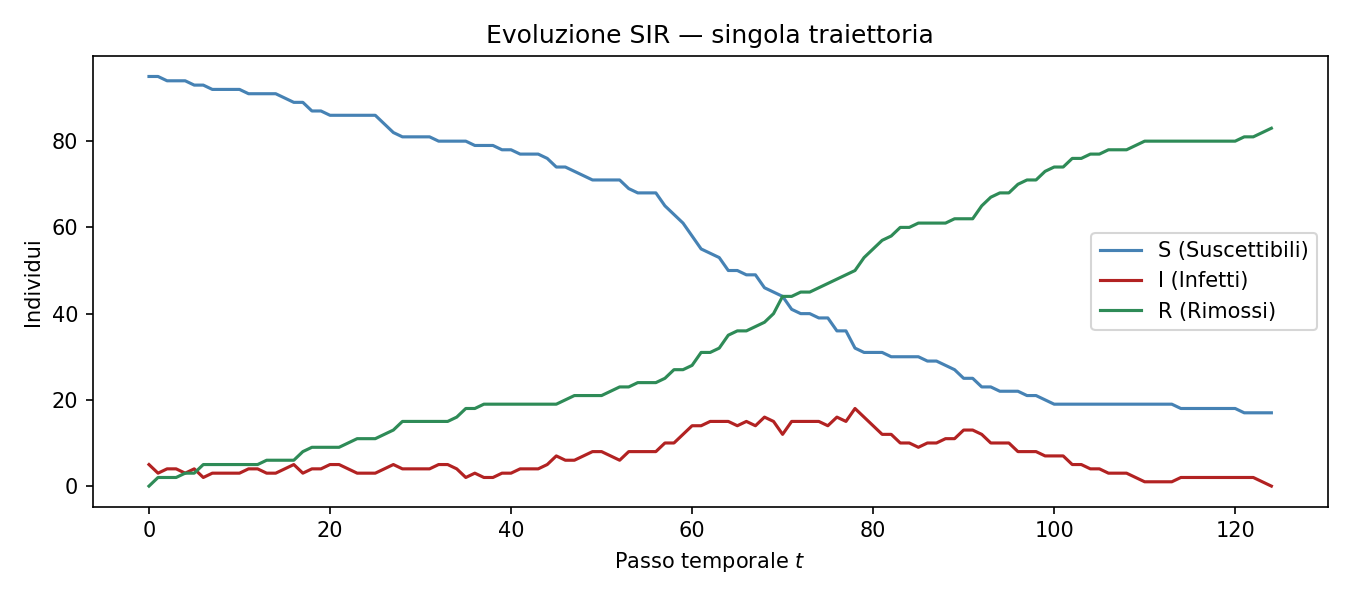
\includegraphics[width=0.74\textwidth]{../img/single_trajectory.png}
\caption{Singola traiettoria stocastica SIR ($N=100, \beta=0.3, \gamma=0.1$): evidenzia le fluttuazioni aleatorie discrete e l'estinzione finale dell'epidemia all'istante $\tau=87$.}
\label{fig:sir_single}
\end{figure}

\begin{figure}[htbp]
\centering
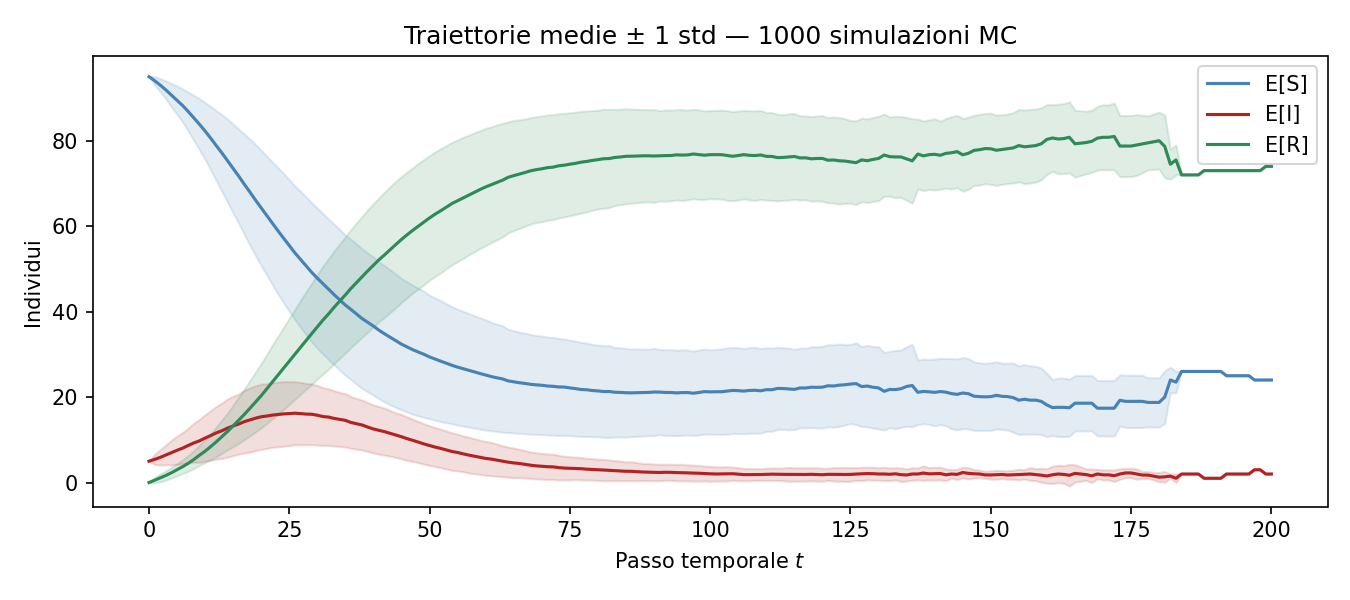
\includegraphics[width=0.74\textwidth]{../img/mean_trajectory.png}
\caption{Traiettoria media su 1000 run Monte Carlo con fascia di confidenza empirica al 95\%.}
\label{fig:sir_mean}
\end{figure}

\begin{figure}[htbp]
\centering
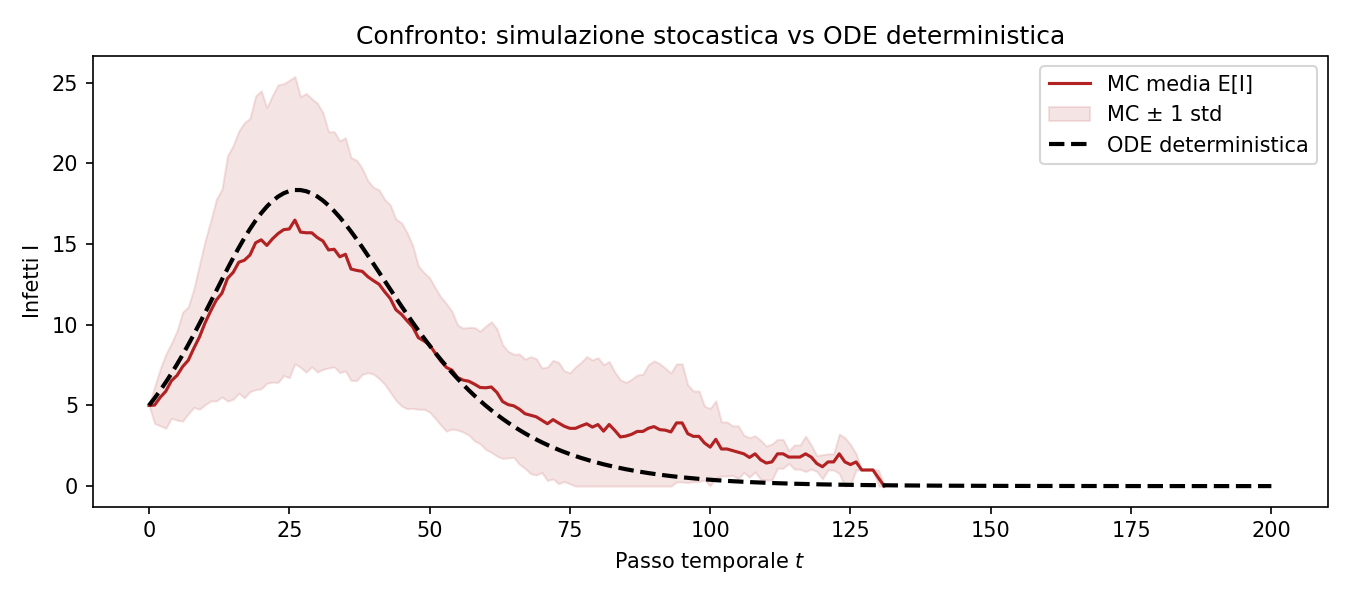
\includegraphics[width=0.74\textwidth]{../img/ode_comparison.png}
\caption{Confronto tra la traiettoria media stocastica reale e l'approssimazione deterministica ODE di Kermack--McKendrick per $N=100$: la stocasticità attenua il picco dell'epidemia dal $30\%$ al $21.94\%$.}
\label{fig:sir_ode}
\end{figure}

\begin{figure}[htbp]
\centering
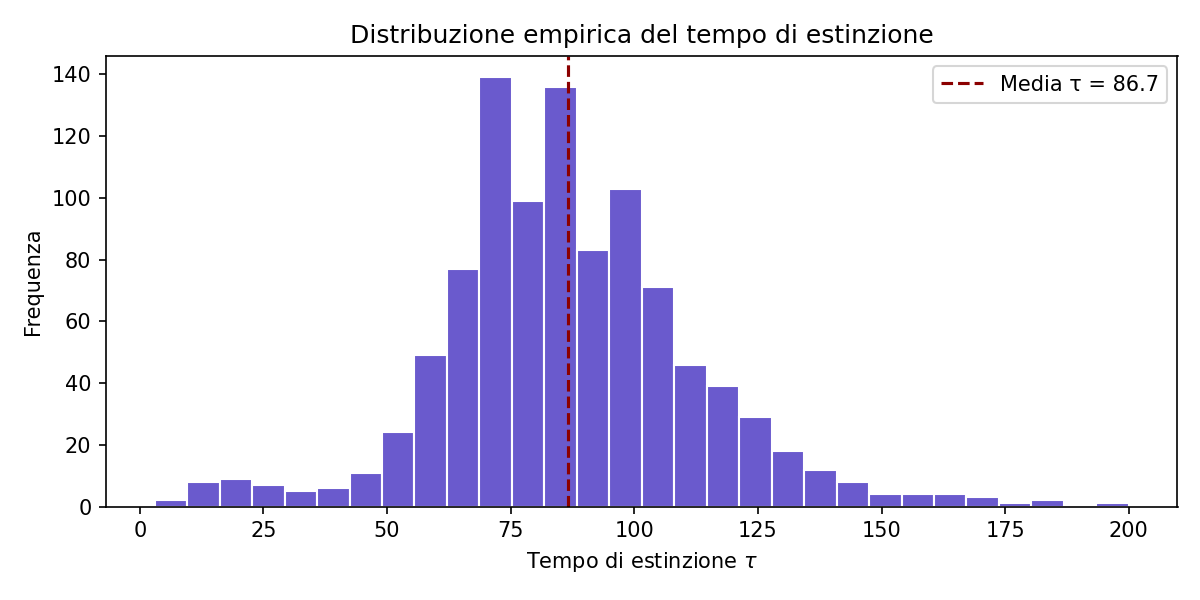
\includegraphics[width=0.72\textwidth]{../img/tau_histogram.png}
\caption{Distribuzione empirica del tempo di estinzione $\tau = \inf\{t : I_t=0\}$ su 1000 simulazioni: media empirica $\bar{\tau} = 86.66$ passi, asimmetria positiva tipica dei tempi di primo assorbimento.}
\label{fig:sir_tau}
\end{figure}

\begin{figure}[htbp]
\centering
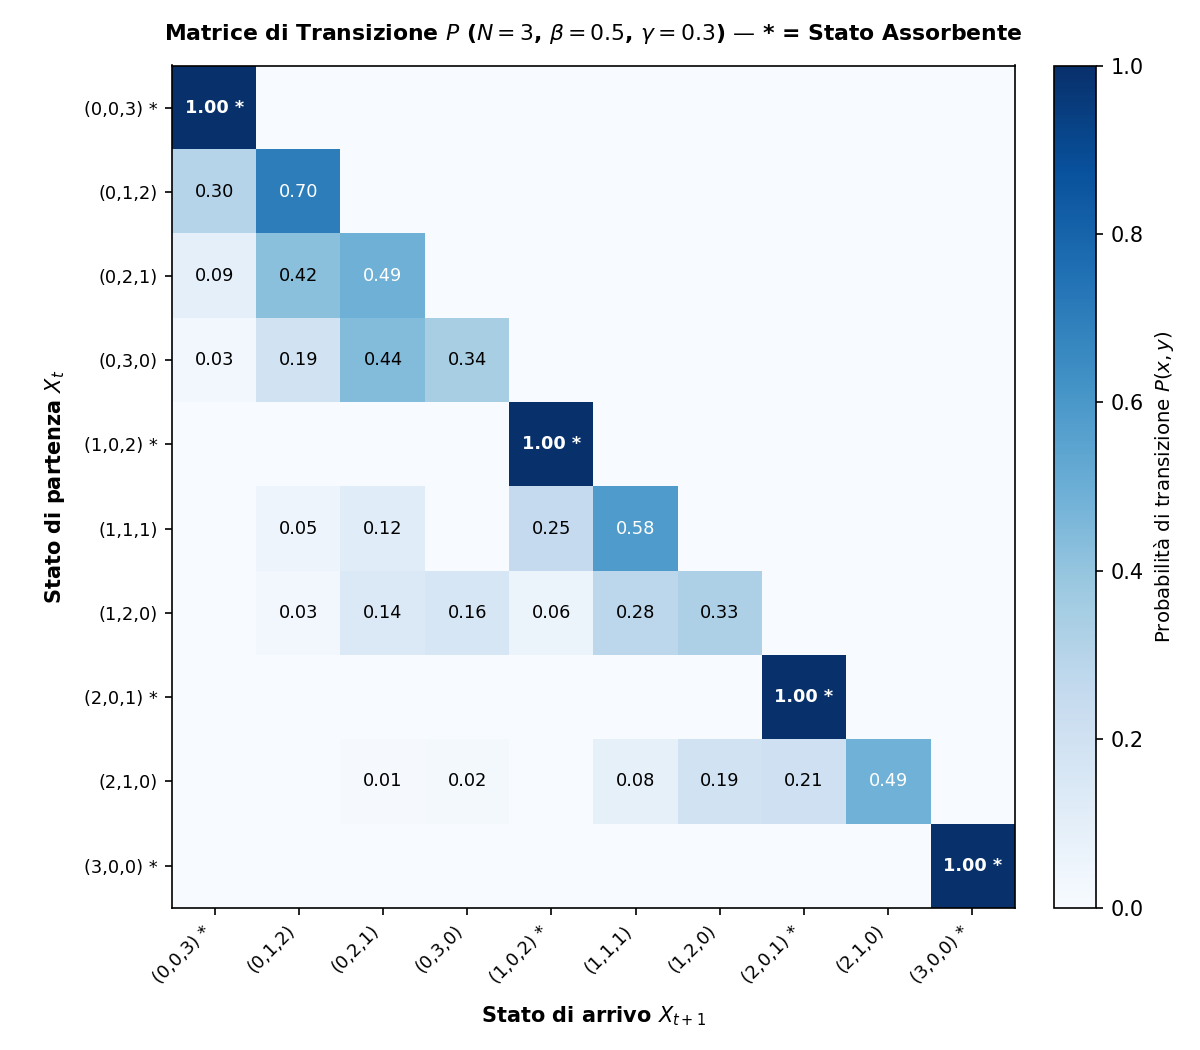
\includegraphics[width=0.72\textwidth]{../img/transition_heatmap.png}
\caption{Heatmap delle probabilità di transizione $p( (s,i) \to (s',i') )$: concentrazione di massa sulle direzioni ammissibili $s' \le s$ e $r' \ge r$.}
\label{fig:sir_heatmap}
\end{figure}

\newpage

% =========================================================================
% CAPITOLO 8: RICHIAMI DI ANALISI E SERIE
% =========================================================================
\chapter{Richiami di Analisi e Serie}

\section{Liminf e Limsup di successioni reali}

Sia $(x_n)_{n \in \N}$ una successione reale. La successione degli estremi inferiori definitivi $y_n := \inf_{k \ge n} x_k$ è crescente, mentre $z_n := \sup_{k \ge n} x_k$ è decrescente.
\begin{definition}[Limite Inferiore e Superiore]
\[ \liminf_{n \to \infty} x_n := \lim_{n \to \infty} \left( \inf_{k \ge n} x_k \right), \qquad \limsup_{n \to \infty} x_n := \lim_{n \to \infty} \left( \sup_{k \ge n} x_k \right) \]
\end{definition}

\begin{spiegazione}[{Perché usiamo $\liminf$ e $\limsup$?}]
    Il limite ordinario può non esistere (es. successioni oscillanti), mentre $\liminf$ e $\limsup$ esistono \textbf{sempre}. Il limite esiste se e solo se $\liminf x_n = \limsup x_n$.
\end{spiegazione}

\section{Serie e Convergenza Assoluta}

\begin{itemize}
    \item \textbf{Serie a termini positivi}: $\sum_{x \in I} f(x)$ converge allo stesso limite indipendentemente dall'ordine dei termini.
    \item \textbf{Serie assolutamente convergenti}: Se $\sum |f(x)| < \infty$, il limite è finito e indipendente dal riordinamento degli addendi.
\end{itemize}

\newpage

% =========================================================================
% APPENDICE: LE 5 DIMOSTRAZIONI D'ESAME DA LAVAGNA
% =========================================================================
\chapter*{Appendice: Le 5 Dimostrazioni d'Esame da Lavagna}
\addcontentsline{toc}{chapter}{Appendice: Le 5 Dimostrazioni d'Esame da Lavagna}

\begin{lavagna}[{1. Dimostrazione: Assorbimento Quasi Certo $\PP(\tau < \infty) = 1$ in Catene Finite}]
\textbf{Tesi}: Se da ogni stato transiente $i \in \mathcal{T}$ è possibile raggiungere un insieme assorbente $\mathcal{A}$ in un numero finito di passi, allora l'assorbimento avviene con probabilità 1.\\
\textbf{Dimostrazione}:
\begin{enumerate}
    \item Sia $m = |\mathcal{T}|$ il numero di stati transienti. Per ogni $i \in \mathcal{T}$, esiste un cammino di lunghezza $\le m$ che porta in $\mathcal{A}$ con probabilità positiva.
    \item Sia $\epsilon = \min_{i \in \mathcal{T}} \PP_i(\tau \le m) > 0$.
    \item La probabilità di trovarsi ancora in $\mathcal{T}$ dopo $k \cdot m$ passi soddisfa la disuguaglianza geometrica:
    \[ \PP_i(\tau > k \cdot m) \le (1 - \epsilon)^k \]
    \item Poiché $1 - \epsilon < 1$, passando al limite per $k \to \infty$:
    \[ \lim_{k \to \infty} \PP_i(\tau > k \cdot m) \le \lim_{k \to \infty} (1-\epsilon)^k = 0 \]
    \item Di conseguenza, $\PP_i(\tau = \infty) = 0 \implies \PP_i(\tau < \infty) = 1$. $\quad \blacksquare$
\end{enumerate}
\end{lavagna}

\begin{lavagna}[{2. Dimostrazione: Invertibilità di $(I-Q)$ e Convergenza della Serie di Neumann}]
\textbf{Tesi}: Se la catena finita è assorbente, allora $Q^k \to 0$ per $k \to \infty$, la matrice $I-Q$ è invertibile e $(I-Q)^{-1} = \sum_{k=0}^\infty Q^k$.\\
\textbf{Dimostrazione}:
\begin{enumerate}
    \item Dall'assorbimento quasi certo, $\lim_{k \to \infty} Q^k = 0$ (la probabilità di restare in $\mathcal{T}$ tende a zero).
    \item Consideriamo il prodotto telescopico parziale:
    \[ (I - Q) \left( \sum_{k=0}^{n-1} Q^k \right) = I - Q^n \]
    \item Facendo tendere $n \to \infty$, poiché $Q^n \to 0$, il membro di destra tende a $I$.
    \item Dunque la serie $\sum_{k=0}^\infty Q^k$ converge e costituisce l'inversa a destra e a sinistra di $I-Q$, ovvero $(I-Q)^{-1} = \sum_{k=0}^\infty Q^k$. $\quad \blacksquare$
\end{enumerate}
\end{lavagna}

\begin{lavagna}[{3. Dimostrazione: Equazioni di Chapman--Kolmogorov $P^{(n+m)} = P^{(n)} P^{(m)}$}]
\textbf{Tesi}: Per ogni $n, m \ge 0$ e stati $i, j \in \mathcal{S}$, si ha $p_{ij}^{(n+m)} = \sum_{k \in \mathcal{S}} p_{ik}^{(n)} p_{kj}^{(m)}$.\\
\textbf{Dimostrazione}:
\begin{enumerate}
    \item Per definizione di probabilità di transizione a $n+m$ passi:
    \[ p_{ij}^{(n+m)} = \PP(X_{n+m} = j \mid X_0 = i) \]
    \item Applichiamo la formula della probabilità totale condizionando rispetto allo stato intermedio $X_n$:
    \[ \PP(X_{n+m} = j \mid X_0 = i) = \sum_{k \in \mathcal{S}} \PP(X_{n+m} = j, X_n = k \mid X_0 = i) \]
    \item Riscriviamo l'intersezione usando la probabilità condizionata:
    \[ = \sum_{k \in \mathcal{S}} \PP(X_{n+m} = j \mid X_n = k, X_0 = i) \cdot \PP(X_n = k \mid X_0 = i) \]
    \item Per la \textbf{Proprietà di Markov}, il futuro a tempo $n+m$ dato il presente a tempo $n$ è indipendente dal passato $X_0 = i$:
    \[ \PP(X_{n+m} = j \mid X_n = k, X_0 = i) = \PP(X_{n+m} = j \mid X_n = k) = p_{kj}^{(m)} \]
    \item Sostituendo:
    \[ p_{ij}^{(n+m)} = \sum_{k \in \mathcal{S}} p_{ik}^{(n)} p_{kj}^{(m)} \quad \blacksquare \]
\end{enumerate}
\end{lavagna}

\begin{lavagna}[{4. Dimostrazione: Tempo Medio di Assorbimento $\mathbf{t} = (I-Q)^{-1}\mathbf{1}$}]
\textbf{Tesi}: Il vettore dei tempi medi di assorbimento $\mathbf{t} = (t_i)_{i \in \mathcal{T}}$ partendo dagli stati transienti soddisfa il sistema lineare $(I-Q)\mathbf{t} = \mathbf{1}$.\\
\textbf{Dimostrazione}:
\begin{enumerate}
    \item Sia $\tau = \inf\{n \ge 0 : X_n \in \mathcal{A}\}$. Per ogni stato transiente $i \in \mathcal{T}$, $t_i = \E_i[\tau]$.
    \item Condizioniamo rispetto al primo passo $X_1$:
    \[ t_i = 1 + \sum_{j \in \mathcal{S}} p_{ij} \E_j[\tau] \]
    \item Separiamo la somma sugli stati transienti $\mathcal{T}$ e assorbenti $\mathcal{A}$:
    \[ t_i = 1 + \sum_{j \in \mathcal{T}} q_{ij} t_j + \sum_{a \in \mathcal{A}} r_{ia} \cdot 0 = 1 + \sum_{j \in \mathcal{T}} q_{ij} t_j \]
    \item In forma matriciale compatta:
    \[ \mathbf{t} = \mathbf{1} + Q \mathbf{t} \iff (I - Q)\mathbf{t} = \mathbf{1} \]
    \item Poiché $(I-Q)$ è invertibile, moltiplicando a sinistra per $(I-Q)^{-1}$:
    \[ \mathbf{t} = (I - Q)^{-1}\mathbf{1} \quad \blacksquare \]
\end{enumerate}
\end{lavagna}

\begin{lavagna}[{5. Dimostrazione: Proprietà della Torre $\E[\E[X \mid \G]] = \E[X]$}]
\textbf{Tesi}: Sia $(\Omega, \F, \PP)$ uno spazio di probabilità e $\G \subseteq \F$ una sub-$\sigma$-algebra. Per ogni $X \in L^1$, si ha $\E[\E[X \mid \G]] = \E[X]$.\\
\textbf{Dimostrazione (Caso di partizione finita $\G = \sigma(A_1, \dots, A_k)$)}:
\begin{enumerate}
    \item Sugli atomi $A_i$ di $\G$, la variabile aleatoria $\E[X \mid \G]$ assume il valore costante $\E[X \mid A_i] = \frac{\E[X \1_{A_i}]}{\PP(A_i)}$.
    \item Calcolando il valore atteso globale della variabile $\E[X \mid \G]$:
    \[ \E[\E[X \mid \G]] = \sum_{i=1}^k \E[X \mid A_i] \PP(A_i) = \sum_{i=1}^k \frac{\E[X \1_{A_i}]}{\PP(A_i)} \PP(A_i) = \sum_{i=1}^k \E[X \1_{A_i}] \]
    \item Per la linearità del valore atteso e sapendo che $\sum_{i=1}^k \1_{A_i} = \1_\Omega = 1$:
    \[ = \E\left[ X \sum_{i=1}^k \1_{A_i} \right] = \E[X \cdot 1] = \E[X] \quad \blacksquare \]
\end{enumerate}
\end{lavagna}

\chapter*{Bibliografia}
\addcontentsline{toc}{chapter}{Bibliografia}
\begin{itemize}
    \item [1] D. Acemoglu, \emph{Introduction to Modern Economic Growth}, Princeton University Press, 2009.
    \item [2] Q. Berger, F. Caravenna, and P. Dai Pra, \emph{Probabilità}, Springer, 2021.
    \item [3] D. Bertsekas, \emph{Dynamic Programming and Optimal Control}, Athena Scientifica, 2005.
    \item [5] P. Billingsley, \emph{Probability and Measure}, Wiley, 1995.
    \item [6] T. Bjork, \emph{Arbitrage theory in continuous time}, Oxford University Press, 2009.
    \item [7] P. Brémaud, \emph{Markov Chains}, Springer, 1999.
    \item [13] S. Federico, \emph{Discrete probability theory with selected topics of discrete time stochastic processes}, Università di Bologna, 2026.
\end{itemize}

\end{document}
